\begin{figure}[!htb]
\centering
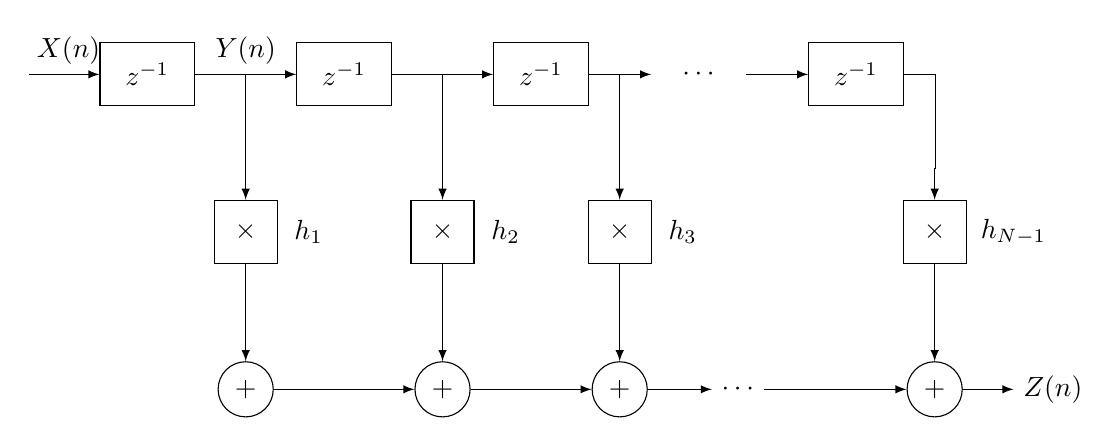
\begin{tikzpicture}[
    auto, 
    node distance=2cm,
    block/.style={rectangle, draw, minimum height=0.8cm, minimum width=1.2cm},
    mult/.style={rectangle, draw, minimum height=0.8cm, minimum width=0.8cm},
    sum/.style={circle, draw, inner sep=0pt, minimum size=0.7cm},
    >=latex
]
% Hauptleitung
% Eingangssignal 
\node at (0.5,0.3) {$X(n)$};

% Erster Verzögerungsblock für Prädiktion
\node[block] at (1.5,0) (pred) {$z^{-1}$};
\draw[->] (0,0) -- (pred.west);

% y(n) nach dem ersten z^{-1} Element
\node at (2.75,0.3) {$Y(n)$};

% Verzögerungselemente nach der Prädiktion
\node[block] at (4,0) (delay1) {$z^{-1}$};
\node[block] at (6.5,0) (delay2) {$z^{-1}$};
\node at (8.5,0) (dots) {$\cdots$};
\node[block] at (10.5,0) (delayN) {$z^{-1}$};

% Durchgehende Pfeile, die direkt zu den Boxen führen
\draw[->] (pred.east) -- (delay1.west);
\draw[->] (delay1.east) -- (delay2.west);
\draw[->] (delay2.east) -- (7.9,0);
\draw[->] (9.1,0) -- (delayN.west);

% Multiplizierer mit X Symbol
\node[mult] at (2.75,-2) (weight0) {$\times$};
\node at (3.55,-2) {$h_1$};
\node[mult] at (5.25,-2) (weight1) {$\times$};
\node at (6.05,-2) {$h_2$};
\node[mult] at (7.5,-2) (weight2) {$\times$};
\node at (8.3,-2) {$h_3$};
\node[mult] at (11.5,-2) (weightN) {$\times$};
\node at (12.5,-2) {$h_{N-1}$};

% Summierer
\node[sum] at (2.75,-4) (sum0) {$+$};
\node[sum] at (5.25,-4) (sum1) {$+$};
\node[sum] at (7.5,-4) (sum2) {$+$};
\node at (9,-4) (dots2) {$\cdots$};
\node[sum] at (11.5,-4) (sumN) {$+$};

% Ausgang
\node at (13,-4) (output) {$Z(n)$};

% Vertikale Verbindungen
\draw[->] (2.75,0) -- (weight0);
\draw[->] (5.25,0) -- (weight1);
\draw[->] (7.5,0) -- (weight2);
\draw[->] (delayN.east) -- ++(0.4,0) -- ++(0,-1.2) -- (11.5,-1.2) -- (weightN.north);

% Verbindungen zu Summierern
\draw[->] (weight0) -- (sum0);
\draw[->] (weight1) -- (sum1);
\draw[->] (weight2) -- (sum2);
\draw[->] (weightN) -- (sumN);

% Verbindungen zwischen Summierern
\draw[->] (sum0) -- (sum1);
\draw[->] (sum1) -- (sum2);
\draw[->] (sum2) -- (dots2);
\draw[->] (dots2) -- (sumN);
\draw[->] (sumN) -- (output);
\end{tikzpicture}
\caption{Prädiktionsfilter}
\end{figure}

\FloatBarrier